\documentclass[a4paper]{report}   % list options between brackets
\usepackage{geometry}
\usepackage{natbib,bibentry}
\usepackage{tocloft}
\usepackage{listings}
\usepackage{verbatim}
\renewcommand\thesection{\arabic{section}}
\setcounter{secnumdepth}{4}
\setcounter{tocdepth}{4}

%table column length
\usepackage{array}
\newcolumntype{L}[1]{>{\raggedright\let\newline\\\arraybackslash\hspace{0pt}}m{#1}}
\newcolumntype{C}[1]{>{\centering\let\newline\\\arraybackslash\hspace{0pt}}m{#1}}
\newcolumntype{R}[1]{>{\raggedleft\let\newline\\\arraybackslash\hspace{0pt}}m{#1}}

% Fonts
\usepackage[T1]{fontenc}
%\usepackage[bitstream-charter]{mathdesign}
\usepackage[scaled=0.85]{beramono}
\usepackage[utf8]{inputenc}






%\usepackage{hyperref,xcolor}
\usepackage{geometry}
\usepackage{natbib,bibentry}
\usepackage{tocloft}

\renewcommand\thesection{\arabic{section}}

% Fonts
%\usepackage[T1]{fontenc}
%\usepackage[bitstream-charter]{mathdesign}
%\usepackage[scaled=0.85]{beramono}
\usepackage[utf8]{inputenc}


\makeatletter
\newif\if@restonecol
\makeatother
\let\algorithm\relax
\let\endalgorithm\relax


\usepackage[linesnumbered,ruled,vlined]{algorithm2e}
\usepackage{epsfig}
\usepackage{graphicx}
\usepackage{caption}
\usepackage{subcaption}
\usepackage{amsfonts}
\usepackage{enumerate}
\usepackage{dsfont}
\usepackage{amsmath}
\usepackage{url}
\usepackage{amssymb}
\usepackage{ifthen}
\usepackage{array}
\usepackage[table]{xcolor}
\usepackage{hyperref}
\usepackage{multirow}
\usepackage{float}
\usepackage{makecell}

%%%%%%%%%%%%%%%%%%%%%%%%%%%%%%%%%%%%%%%%%%%%%%
% content macro
%%%%%%%%%%%%%%%%%%%%%%%%%%%%%%%%%%%%%%%%%%%%%%
\newcommand{\Targetsys}{SoSS}
\newcommand{\Targetsyss}{SoSS}
\newcommand{\targetsyss}{SoSS}
\newcommand{\targetsys}{SoSS}
\newcommand{\rulesep}{\unskip\ \vrule\ }

%%%%%%%%%%%%%%%%%%%%%%%%%%%%%%%%%%%%%%%%%%%%%%
% math macro
%%%%%%%%%%%%%%%%%%%%%%%%%%%%%%%%%%%%%%%%%%%%%%
\newcommand{\inp}{x}
\newcommand{\inpseq}{{\bf x}}
\newcommand{\f}{{\bf f}}
\newcommand{\q}{{\bf q}}
\newcommand{\blab}{{\bf \lab}}
\newcommand{\lab}{y}
\newcommand{\labs}{{\bf y}}
\newcommand{\nlab}{{\bar y}}
\newcommand{\loss}{L}
\newcommand{\expect}[1]{\mathbb{E}_{X,Y}\bigl[#1 \bigr]}

\newcommand{\fscore}{f}
\newcommand{\score}{s}
\newcommand{\SGDloss}{L_\obs(\fscore_{w(t)}(\obs_t), \labs_t)}
\newcommand{\len}[1]{{[#1]}}
\newcommand{\pair}[1]{(\inpseq_{#1},\lab_{#1})}
\newcommand{\npair}[1]{(\bar \inpseq_{#1},\bar \lab_{#1})}
\newcommand{\pairloss}{l_p(\fscore_w(\inp_i)-\fscore_w(\bar \inp_j))}
\newcommand{\pairlossArg}[1]{l_p({#1})}
\newcommand{\slossnew}{\Psi}
\newcommand{\bbeta}{\boldsymbol{\beta}}
\newcommand{\bs}{{\bf s}}
\newcommand{\boldr}{{\bf r}}

\newcommand{\qm}{{\tt r}}

\newcommand{\pospart}[1]{\left [ #1 \right ]_+}

%%%%%%%%%%%%%%%%%%%%%%%%%%%%%%%%%%%%%%%%%%%%%%%%%%%%%%
%   framework
%%%%%%%%%%%%%%%%%%%%%%%%%%%%%%%%%%%%%%%%%%%%%%%%%%%%%%

\newcommand{\lenq}[1]{|#1|}

\newcommand{\subsetOfQuery}[1]{{\cal S}(#1)}
\newcommand{\set}[1]{\left \{ #1 \right \}}
 \newcommand{\sset}[1]{\bigl \{ #1 \bigr \}}
\newcommand{\bigpospart}[1]{\Big [ #1 \Big ]_+}
\newcommand{\norm}[1]{\left | \left | #1 \right | \right |}
\newcommand{\indic}[1]{I_{\set{#1}}}
\newcommand{\expobs}{\expectation_{(\obs, \rels) \sim \mu}}

\newcommand{\expmu}{\expectation_{\inpseqb \sim \mu}}
\newcommand{\empexpmu}{\empexpectation_{\inpseqb \sim \trset}}
\newcommand{\expnu}{\expectation_{\inp \sim \nu}}

\DeclareMathOperator*{\argmax}{arg\,max}
\DeclareMathOperator*{\argmin}{arg\,min}
\DeclareMathOperator*{\argsort}{arg\,sort}
\DeclareMathOperator{\indicc}{I\!I}
\DeclareMathOperator{\nindicc}{I\!I\!I}
\DeclareMathOperator{\dist}{d}
\DeclareMathOperator*{\expectation}{\mathbb{E}}

\newcommand{\probasobs}{\probas\left({\cal S}\right)}
\newcommand{\expxy}{\expectation_{X,Y}}
\newcommand{\expx}{\expectation_{X}}

%%%%%%%%%%%%%%%%%%%%%%%%%%%%%%%%%%%%%%%%%%%%%%%%%%%%%%%%%%%%%%%%%%%%%
% textimage retrieval macro
%%%%%%%%%%%%%%%%%%%%%%%%%%%%%%%%%%%%%%%%%%%%%%%%%%%%%%%%%%%%%%%%%%%%%
\newcommand{\params}{{\bf w}}
\newcommand{\trset}{S}
\newcommand{\alts}{{\bf X}}
\newcommand{\alt}{X}
\newcommand{\emploss}{\hat{R}^{\rerr}(\score, S)}
\newcommand{\dotp}[2]{\left<#1, #2\right>} %dot product
\newcommand{\intint}[2]{\set{#1, ..., #2}}%{\left \{#1..#2\right \}}
\newcommand{\sign}{\mbox{sign}}
%\newcommand{\pospart}[1]{\left [ #1 \right ]_+}
\renewcommand{\Re}{\mathbb{R}}
%\DeclareMathOperator{\indic}{I}
\DeclareMathOperator*{\empexpectation}{\hat{\mathbb{E}}}
\newcommand{\empexpobs}{\empexpectation_{(\obs, \rels) \sim \trset}}
\newcommand{\rel}{y}
\newcommand{\nrel}{{\bar y}}

% Spaces
\newcommand{\fspace}{{\cal F}}
\newcommand{\hfspace}{{\cal H}}
\newcommand{\inpspace}{{\cal X}}
\newcommand{\supspace}{{\cal Y}}
\newcommand{\distspace}{{Pr(X,Y)}}
\newcommand{\distspacex}{{Pr(X)}}
\newcommand{\alldistspace}{{\cal D}}


%%%%%%%%%%%%%%%%%%%%%%%%%%%%%%%%%%%%%%%%%%%%%%
% code for formatting comments
%%%%%%%%%%%%%%%%%%%%    BEGIN  %%%%%%%%%%%%%%%%%%%%
\newboolean{showcomments}
\setboolean{showcomments}{false}

\ifthenelse{\boolean{showcomments}}
{ \newcommand{\mynote}[2]{
    \fbox{\bfseries\sffamily\scriptsize#1}
    {\small$\blacktriangleright$\textsf{\emph{#2}}$\blacktriangleleft$}}}
{ \newcommand{\mynote}[2]{}}

\newcommand{\guthemberg}[1]{\mynote{Guthemberg}{#1}}
%%%%%%%%%%%%%%%%%%%%    END  %%%%%%%%%%%%%%%%%%%%



%%%%%%%%%%%%%%%%%%%%END%%%%%%%%%%%%%%%%%%%%%%%







\begin{document}

	\begin{figure}
	    			%\centering
	    			
\includegraphics[scale=0.45]{inputs/img/svc}
	  		\end{figure}

%Investissement d'Avenir Développement de l’Économie Numérique
%``Informatique en nuage''
\title{Deliverable 4.1.3.1 -- \emph{Prototype de prévision des défaillances et expérimentations}}   % type title between braces
\author{List of authors HERE}         % type author(s) between braces
\date{30 September 2015}    % type date between braces
\maketitle

\begin{abstract}
This document describes the progress made within Task 4.2.B ``Évaluation de la sûreté de fonctionnement : Mise en œuvre et expérimentations''  over the last year of the SVC project,  and in this respect it complements
deliverable 4.1.2.2.  In this deliverable, we detail the design, installation, and set-up of the Tejo prototype, an anomaly detection scheme for cloud databases. We also describe our latest experimental set-up and results with Tejo in our private cloud.


\end{abstract}

\tableofcontents

\newpage
\listoffigures
\newpage
\listoftables
\newpage


\section{Introduction}

Big data has transformed the way we manage information. As an unprecedented volume of data has become available, there is an increasing demand for stream processing platforms to transform raw data into meaningful knowledge. These velocity-oriented platforms may rely on cloud databases to provide fast data management of continuous and contiguous flows of data with horizontal scalability. Therefore, cloud databases represent an important technology component for a broad range of data-driven domains, including social media, online advertisement, financial trading, security services, and policy-making process.

The architecture of row-store-based relational databases has evolved to meet the requirements of big data on the cloud~\cite{ren2012lightweight}, like elasticity, data partitioning, shared nothing, and especially high performance. The so-called NewSQL databases offer high-speed, scalable data processing in main-memory with consistency guarantees through ACID (atomicity, consistency, isolation, and durability) transactions.

To ensure fast data management, NewSQL databases rely on built-in, fault tolerance mechanisms, like data partitioning, replication, redundant network topologies, load balancing, and failover. Although these mechanisms handle fail-stop failures successfully, many other cloud performance anomalies may remain unnoticed~\cite{server_delays}. For instance, Do \emph{et al.}~\cite{do2013limplock} found that a single limping network interface can cause a three orders of magnitude execution slowdown in cloud databases. Therefore, we believe that the dependability of NewSQL databases might be improved by detecting these anomalies. 

This document proposes Tejo, a supervised anomaly detection scheme for NewSQL databases. We make three specific contributions. First, we introduce a scheme for analysing performance anomalies using fault injection tools and a supervised learning model. Second, we shed some light on the impact of performance anomalies in NewSQL databases. Third, we highlight the importance of selecting the proper features and statistical learning algorithm to enhance the anomaly detection efficiency on these databases.

In the next section, we lay out the recent trends in data stream processing and anomaly detection with statistical learning. Following this, in Section 3 we describe the design of Tejo, in particular its components and its two-phased functioning, namely learning and detection phase. In Section 4 we evaluate VoltDB, a prominent NewSQL database, using Tejo. In our experimental setup, VoltDB served two workloads, whose data was partitioned and replicated across a cluster of virtual machines (VMs). A similar set-up might be done for a MongoDB cluster, as presented in our previous work~\cite{silvestre2014anomaly}. Finally, we discuss the related work in Section 5, and conclude in Section 6.



\section{Related Work}
\label{sec:related_work}

\noindent
{\bf Fault tolerance in distributed databases.} \ Distributed databases use replication and advanced request scheduling to improve data availability. Bayou~\cite{petersen1996bayou} is data storage that relies on replication to ensure data availability against fail-stop failures, but they are not able to deal with performance anomalies. Skute~\cite{bonvin2010self} provides an adaptive replication scheme that mitigates the impact of performance anomalies. However, it does not provide mechanisms to ensure high data availability, such as high throughput and bounded latency. Emerging cloud databases, like VoltDB and MongoDB, offer high data availability using enhanced main memory data structures~\cite{stonebraker2010sql}. But, our findings of this and previous study~\cite{silvestre2014anomaly} show that performance anomalies on the cloud, including malfunctioning network cards, disk and main memory, can undermine the performance of cloud databases. 

Cake~\cite{wang2012cake} offers a scheduling scheme to enforce high-level data availability requirements for end users. However, Cake was not designed to identify faulty VMs. Eriksson \emph{et al.}~\cite{eriksson2013riskroute} provide a routing framework that helps cloud operators to mitigate the impact of network failures. We believe that our work is complementary to theirs. Alerts from Tejo about anomalies in network, memory, disk and CPU of VMs, can contribute to enhance the efficiency of such scheduling mechanisms.

\noindent
{\bf Anomaly detection with statistical learning.} \ Anomaly detection is commonly implemented based on an \emph{unsupervised learning method}. Gujrati \emph{et al.}~\cite{gujrati2007meta} provide prediction models based on event logs of supercomputers to detect platform-wide anomalies, whereas we are interested in detecting anomalous VMs based on monitoring data. Chen \emph{et al.}~\cite{chen2007failure} propose an anomaly detection approach for large-scale systems that improves the prediction efficiency of an entropy-based information theory technique by performing a principal component analysis (PCA) of system inputs. However, this introduces computational overhead that undermines its scalability and causes a slowdown in anomaly predictions. While we focus on detecting performance anomalies in NewSQL databases, Lan \emph{et al.}~\cite{lan2010toward} provide a general-purpose anomaly detection approach that relies on features selection to enhance prediction efficiency. Similarly, Guan and Fu~\cite{guan2013adaptive} perform feature extraction based on PCA to identify the most relevant inputs for anomaly detection. Yet, results of our previous work~\cite{silvestre2014anomaly} confirm that a supervised method with all features outperforms a unsupervised one by reducing the number of false positives by 10\%. In this work, we extended our previous supervised learning model to detect multiple classes of anomalies based on SLO metrics.

Guan \emph{et al.}~\cite{guan2012cda} implement a probabilistic prediction model based on a \emph{supervised learning method}. Although their model allows us to compare the dependability of virtualized and non-virtualized cloud systems, it suffers from poor prediction efficiency when it is used to predict cloud performance anomalies. Tan \emph{et al.}~\cite{tan2012prepare} propose general-purpose prediction model to prevent performance anomalies. Their \emph{supervised learning}-based model combines 2-dependent Markov chain model with the tree-augmented Bayesian networks. But, the authors did not provide information about the prediction efficiency and the capacity of their approach to generalize. We show with Tejo that the choice of the learning algorithm and features contribute to enhance predictive efficiency of performance anomalies.

\section{Background}
\label{sec:background}


\subsection{Big data stream processing and NewSQL databases}

To processing continuous streams of big data, we consider the emerging stream processing platforms~\cite{leskovec2014mining}, as depicted in Figure~\ref{fig:newsql_data_stream}. In these platforms, streams of data are processed by two complementary systems: the fast stream processing system and big archival engine. The former manages high-speed data streams to provide real-time analytics and data-driven decisioning, providing services like fraud heuristics, market segmentation, or optimal customer experience; while the later computes huge volumes of historical data for long-term data analytics, such as scientific results, seasonal predictions, and capacity planning. Big archival engines are built on data warehouse technologies like Hadoop and column-stores. In contrast, fast stream processing technologies are still emerging. Among these technologies are NewSQL databases like VoltDB~\cite{stonebraker2013voltdb} and S-Store~\cite{cetintemel2014s}. To support incremental, stateful ingest of data streams into a scalable system, NewSQL databases provide low-latency via in-memory distributed processing and a strong support for transaction management with ACID guarantees. However, as NewSQL databases are deployed on cloud infrastructures to scale to large clusters, cloud performance anomalies may undermine their capacity of fast stream processing.

\begin{figure}[!h]
  \centering
     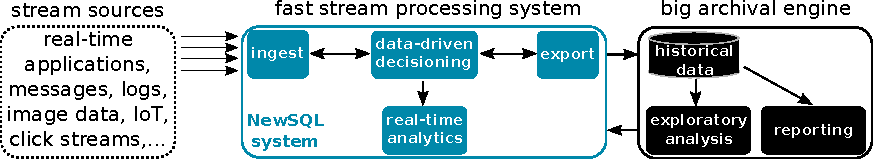
\includegraphics[width=.8\textwidth]{inputs/img/simple_newsql_data_stream}
  \caption{The emerging stream processing platforms for big data.}
  \label{fig:newsql_data_stream}
\end{figure}

\subsection{Anomaly detection using statistical learning}
\label{subsec:anomaly}

Statistical learning has been a widely used technique to predict performance anomalies in large-scale distributed systems~\cite{chandola2009anomaly}. It makes prediction by processing feature vector $\inpseq$ with a fixed
  number of dimensions $d$ ($\inpseq \in \inpspace \subset \Re^d$) from the input space $\mathcal{X}$. There are two main methods: \emph{supervised} and \emph{unsupervised learning}. 

The \emph{supervised learning method} couples each input with a $\rel$, a label, from the output space  $\mathcal{Y}$. To learn, we have $N$ pairs ($\inpseq,\rel$) drawn \emph{independent and identically distributed} (i.i.d.) from a fixed but unknown joint probability density function $\distspace$. This method searches for a function $\fscore$ : $\mathcal{X} \rightarrow \Re$  in a fixed function class $\fspace$ in the learning dataset. State-of-the-art algorithms, like \emph{random forests}~\cite{breiman2001random}, aim to find $\fscore^\star$ in $\fspace$ with the lowest empirical risk $\fscore^\star \in \argmin_{\fscore \in \fspace} \qm_{emp}(\fscore)$,
where $\qm_{emp}(\fscore) = \frac{1}{N} \sum_{i=1}^N \indic{\fscore(\inpseq) \neq \lab_i}$ is computed over the training set, and $\indic{.}$ is the indicator function which returns $1$ if the predicate $\{.\}$ is true and $0$ otherwise. Similarly, an \emph{unsupervised learning method} relies on $N$ unlabelled samples having probability density function $\distspacex$. Unlike supervised learning, predictions provide insights into how the data is organized or clustered.

Most of the anomaly detection approaches for distributed systems are based on a general-purpose, unsupervised learning method~\cite{gujrati2007meta,lan2010toward,guan2013adaptive}. However, prediction efficiency remains the main drawback of this method~\cite{love2002comparing}. Results in our previous work~\cite{silvestre2014anomaly} confirm that a supervised learning method overcomes an unsupervised one in cloud anomaly detection. In this work, we extend our supervised learning model as a component of Tejo to classify anomalous VMs in four different classes.

\section{Design}
\label{sec:design}

Tejo comprises three components, namely a set of fault injection tools, a data handler, and a learning model. These components interoperate into two distinct phases: learning and detection phase. While the first phase allows us to evaluate the performance of a NewSQL database under anomalies, the second permits the detection of these anomalies. Figure~\ref{fig:tejo_overview} depicts the components and the two-phase functioning of Tejo.


\begin{figure*}
        \centering
        \begin{subfigure}[b]{0.48\textwidth}
               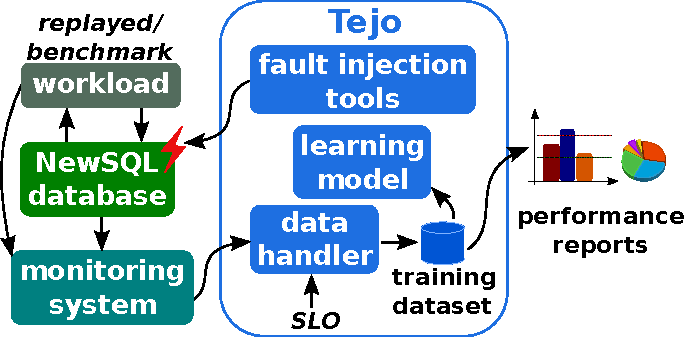
\includegraphics[width=1\textwidth]{inputs/img/tejo_overview_learning_newsql}
                \caption{Learning phase.}
                \label{fig:tejo_overview_learning}
        \end{subfigure}
	\rulesep
        \begin{subfigure}[b]{0.48\textwidth}
                  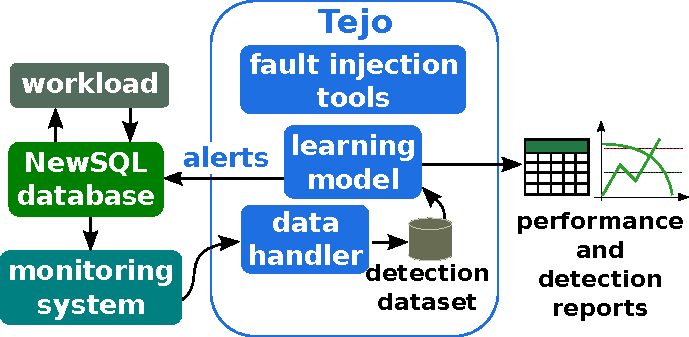
\includegraphics[width=1\textwidth]{inputs/img/tejo_overview_detection_newsql}
                \caption{Detection phase.}
                \label{fig:tejo_overview_detecting}
        \end{subfigure}
        \caption{Tejo operates in two distinct phases: learning and detection phase.}\label{fig:tejo_overview}
\end{figure*}

\subsection{The components of Tejo}
\label{subsec:tejo_components}

\subsubsection{Fault injection tools.} 
To provoke performance anomalies, this component emulates four categories of faulty events in VMs of a NewSQL database cluster. 

\emph{Network faults}. Communication issues are common in distributed systems. To analyse their impact, we inject three types of network faults, namely packet loss, network latency, and limping network. Packet loss and network latency emulates interconnection issues, such as network partition. Limping network reproduces anomalies previously observed by Do \emph{et al.}~\cite{do2013limplock}, where the transmission rate of limping network interface is smaller than the manufacturer's specification. 

\emph{Memory faults}. As NewSQL databases fit the entire data to the main memory, they become more vulnerable to anomalies in memory availability. To provoke such anomalies, we make arbitrary amounts of main memory unavailable. As a result, the database instance is likely to perform more costly disk I/O operations. A typical example of this fault is a VM running out of memory due to a misconfiguration, memory leaking, overloading, or an unbalanced resource allocation.

\emph{Disk faults}. Although most NewSQL databases manage data in main memory, disk-intensive processes may have an impact of its performance. This category of fault emulates an arbitrary number of jobs performing several disk operations, including writes, reads, and file syncs.  

\emph{CPU faults}. CPU is a key resource in a virtual machine. As unattended number of processes compete the database instance to CPU resources, they may undermine the performance of the database cluster. The CPU fault emulates an arbitrary number of jobs performing arithmetic operations to overload the VM cores. 


\subsubsection{The data handler.} 
This component computes data from the monitoring system (i) to collect the performance counters of a NewSQL database and (ii) to provide data to characterize performance anomalies.

\emph{Collect the performance counters of a NewSQL database}. The data handler samples monitoring data to collect the current state of the NewSQL cluster, as depicted in Figure~\ref{fig:tejo_overview}. To this end, it frequently communicates with the monitoring system to fetch raw monitoring data and to convert it into useful, aggregated information. The content of the resulting aggregated information depends on the aim of each functioning phase, learning or detection, detailed below. 

\emph{Providing data to characterize performance anomalies}. After aggregating samples of monitoring data, the data handler organizes this data into \emph{feature vectors}. These vectors represent the state of the VMs of the database cluster or the workload. The vectors are stored in datasets for performance analysis or anomaly detection. 

\subsubsection{The learning model.} 
The learning model is at the heart of the Tejo scheme. The purpose of this model, the so-called predictive task, is to characterize the behaviour of VMs under performance anomalies. Given an i.i.d. sample $(\inpseq,\rel)$, described in Subsection~\ref{sec:background}, we model our predictive task as a classification problem, whose inputs and outputs are defined as follows.

\emph{Inputs}. We represent the input space $\inpseq$ as a VM running a database instance. This input data corresponds to a feature vector computed by the data handler component. The size of the feature vector matters. In general, the higher the dimension of this vector, the higher the predictive efficiency is. However, an increase in the input dimension rises the computational cost of predictions.

\emph{Outputs}. The supervision $\rel$ associated to each input VM $\inpseq$ is based on five possible classes, $\mathcal{Y} \in \{0,1,2,3,4\}$, whose labels are \emph{normal}, \emph{network-related anomaly}, \emph{memory-related anomaly}, \emph{disk-related anomaly}, and \emph{CPU-related anomaly} respectively. Depending on the phase of Tejo (detailed below), these labels are assigned by either computing the training dataset or by a learning algorithm.

\subsection{Two-phase functioning}
\label{subsec:tejo_phases}

\subsubsection{Learning phase.} In this phase, Tejo learns the behaviour of the database cluster under anomalies and reports on its performance.

\emph{Requirements}. As illustrated in Figure~\ref{fig:tejo_overview_learning}, Tejo relies on an already existing monitoring system to poll performance counters from both VMs and workload. To measure the cluster-wide performance counters, we assume that the workload can be replayed or run through a benchmark tool. We consider that Tejo's analyst specifies expected SLO metrics, such as average throughput and $99^{th}$ percentile latency. The analyst must also specify parameters of the fault campaign and running experiments, including intensity and duration of each fault, number of injections, and interval between consecutive fault injections. 

\emph{Functioning.} As the replayed/benchmark workload runs, the fault injection tool performs a fault injection campaign to emulate performance anomalies. Meanwhile, performance counters from both the workload and VMs running the database cluster are collected by the monitoring system and computed by the data handler component. As the data handler computes the monitoring data in feature vectors, it adds information about injected faults and labels. Labels correspond to output classes of learning model and are added with respect to SLO metrics. The feature vectors are then stored in the training dataset. After running the workload and accomplishing the fault injection campaign, the learning model computes the feature vectors of VMs from the training dataset.

\emph{Reports.} Besides providing data to learn the behaviour of anomalous VMs, analysts can observe the impact of anomalies in the throughput and $99^{th}$ percentile latency. They may evaluate which anomalies cause SLO  violations, gaining more insight into the efficiency of existing fault-tolerance mechanisms. 

\subsubsection{Detection phase.} In this phase, Tejo reports on the efficiency of the learning model and performs anomaly detection in VMs at runtime. 

\emph{Requirements}. Similar to the training phase, Tejo relies on an existing monitoring platform to gather data for predictions. It requires that the learning model has already been trained as detailed in learning phase described above. We assume that SLO targets and the workload are the same as those of the learning phase. 

\emph{Functioning.} While the NewSQL database serves the workload, the data handler gathers the monitoring data and creates feature vectors of VMs in the detection dataset. As soon as a new feature vector is created, the learning model computes it to detect performance anomalies whenever they occur.  

\emph{Reports.} Tejo's learning model predicts labels of incoming feature vectors. Then alerts are generated about detected anomalies. These alerts may be handled by the database to trigger recovery procedures. Besides generating alerts, it reports on the efficiency of the learning model, including comparing different learning algorithms, ranking performance counters with regard to their importance, calculating the computational cost, and verifying model over-fitting  or under-fitting. 


\section{Prototype set-up}

In this section we describe the set-up of Tejo in a cloud platform. Initially, we detail the basic roles of nodes in Tejo design through a simple topology that guides us throughout this section. Then we list the steps to install nodes according to their roles and requirements. We also provide some guidelines to the installation of cloud databases, useful for validation purposes. After the installation steps, we explain how to configure nodes to work as part of Tejo.

\subsection{Role of nodes in Tejo and their main interactions}
\label{subsec:roles}

Nodes play specific roles according to the services they provide to the anomaly detection scheme. There are thee main roles:

\begin{itemize}
	\item Service Unity (SU): This is the node, commonly a virtual machine, whose services are observed by Tejo in order to identify anomalous behaviours. Essentially, SU runs processes, commonly from a distributed system, whose performance might be undermined by undesired cloud behaviours. Therefore, each SU provides monitoring information to characterize the performance of the process running on it. When Tejo orchestrates fault injection campaigns, SUs actually run scripts that emulate faults. In this document, we focus on clusters of cloud databases where the components of the cluster, SUs, play a role of data storage process. However, we assume that the vast majority of monitoring data provided by SU is not specific to cloud databases, hence Tejo is flexible enough to detect anomalies in other distributed services deployed in cloud platforms.
	\item Workload: Nodes that play a role of Workload generate requests to the service running atop SUs. Essentially, they emulate the service load, similar to that expected in the real deployment, that SUs should serve. This role allows us to reproduce the behaviour of users and to verify if their expectations are met through service level objectives monitoring. When Tejo runs in production it is represented by remote requests from clients. 
	\item Monitor: This is the main role of Tejo scheme. In this role, data for anomaly detection is collected from different sources (SUs and Workloads), computed, and stored in a SQL database. This node also runs routines to learn or predict anomalous behaviour from the collected data, playing a key role to send alerts about anomalous SUs. 
\end{itemize} 

The Figure~\ref{fig:roles_scheme} depicts the main roles and interactions of Tejo prototype through a simplified scheme. It highlights the main Tejo's services that run atop each role and how they exchange data. For instance, the SU plays a key role by running the cloud database. SU also runs the fault injection tools, which are orchestrated by the monitor machine (following the arrow from the data handler in Monitor towards SU), and a monitor agent that allows us to collect data about the functioning of the SU. This monitoring data is aggregated by the monitor system running on Monitor, which is also able to aggregate monitoring data from the Workload.


\begin{figure}[!h]
  \centering
     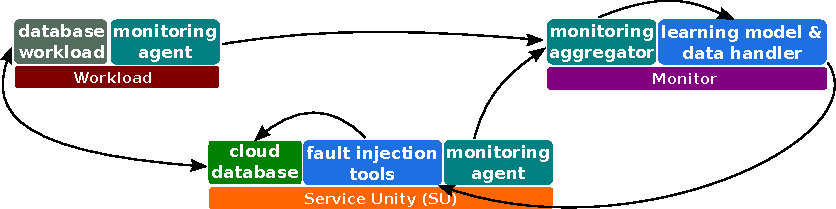
\includegraphics[width=1\textwidth]{inputs/img/roles_scheme}
  \caption{Main roles and interactions of Tejo prototype.}
  \label{fig:roles_scheme}
\end{figure}


\subsection{Installation}

In this subsection, we describe the main installation steps of our prototype. Our description will be based on the scheme depicted in Figure~\ref{fig:roles_scheme} and is organized as follows. First, we provide an overview of the installations tools available online. In turn, we describe the installation steps that are common to all roles. Then we describe installation steps that are specific to the roles, explaining the main steps to set-up a Monitor. After the Monitor set-up, we describe the installation of a SU and finally the installation of the Workload.

\subsubsection{Installation scripts and source code organization in the publicly available repository}
\label{subsubsec:gitclone}

All the scripts to perform the installation of the prototype of Tejo are available online~\footnote{An anomaly detection scheme for cloud databases: \url{https://github.com/guthemberg/tejo}}.  To start installing Tejo, retrieve the all sources from the online repository as follows:


\begin{lstlisting}
git clone https://github.com/guthemberg/tejo
\end{lstlisting}


Overall, the repository is organized in the following way.

\lstinputlisting[language=sh, firstline=1, lastline=22,frame=single]  {inputs/sources/repo_organization.txt}

There are two folders in the repository root: \verb|contrib| and \verb|tejo|. \verb|contrib| has a collection of scripts necessary to the installation procedure organized by operating system distribution and packages specificities. As we will explain in futher details in the following subsections, most of packages required to install our prototype are available on any unix-like system. However, for a matter of simplicity, we have adapted the installation scripts to be more comfortably performed in Debian systems, more precisely, to the 7.8 release. This includes all scripts and configuration files templates available inside \verb|contrib/debian|, which might be easily modified for other distributions. In \verb|contrib|, we provide a set of tools and templates to install Workload role in fedora-like systems, particularly customized for PlanetLab testbed. Moreover, one will find binaries of \verb|paping|~\footnote{paping: Cross-platform TCP port testing, emulating the functionality of ping (port ping). \url{https://code.google.com/p/paping/}}, a tcp-based tool for latency measurements, a template of the main configurations file of Tejo along with some of its miscellaneous/tuning scripts.

While \verb|contrib|  mostly provides installation scripts for third-party, required packages, \verb|tejo| has the main sources and modules of our prototype itself. It contains four directories: \verb|common|, \verb|data_handler|, \verb|fault_injection_tools|, and \verb|learning_model|. The first one has a collection of commonly performed tasks as Tejo runs, such as launching experiments and fault injection campaigns as well as monitoring database set-up scheme and backup. The latter three directories correspond pretty much to the modules described in Section~\ref{sec:design}. They actually provide the main functionalities of our prototype, including computing the monitoring data, fault injection campaign orchestration and learning/predictions of anomalies.

\subsubsection{Common installation steps}

Regardless the role of the node, we should perform a few preliminary installation steps to set-up Tejo. These steps mainly concern a set of common installation packages and some adjustments to configuration files. Table~\ref{tab:common_install_conf_node} concisely describes these steps and the configuration file templates to be customized.

			\begin{table*}[htdp]
				\begin{center}
\caption{Common required packages and main configuration file.}
  \label{tab:common_install_conf_node}
					\begin{tabular}{R{2.5cm} || L{4.5cm} L{6cm} }
						{\bf Requirement}&{\bf Template/packages}&{\bf Description} \\  
						\hline
						\hline
						{\bf Common packages}&rcconf sysv-rc-conf wget ntp ntpdate rdate screen htop apt-show-versions ethtool gcc git nmap less iperf bc tcsh & This list provides a common set of open-source packages required by the collection of Unix shell scripts of Tejo.\\
						\hline
						{\bf Python libraries/tools}&python-psutil python-pip python-configobj python-dev python-rrdtool python-psycopg2 & Most of scripts of Tejo are implemented in Python language, notably those that provide interface to database API, configuration file parsing, interface to monitoring data database API (rrd), etc.\\
						\hline
						{\bf Java}&openjdk-7-jdk & Several functionalities of Tejo require java (release 7 or higher) support, e.g. workload generator and query router/load balancer.\\
						\hline
						{\bf The main configuration file}&\verb|tejo/contrib/tejo/| \verb|tejo.conf.sample|&This file provides the main parameters for Tejo functioning and should be copied to \verb|/etc| directory. This file contains a couple of keywords in upper-case letters to be replaced/customized accordingly. At this point of the installation, the key words to be customized are: USER, GUEST\_PASSWORD, and MY\_DOMAIN.  \\
					\end{tabular}
				\end{center}
			\end{table*}



\subsubsection{Installing a Monitor node}

Monitor is the main role of Tejo prototype. As briefly described in Subsection~\ref{subsec:roles}, a node that plays this role is in charge of (i) aggregating and computing monitoring data, (ii) orchestrating fault injection campaigns and (iii) predicting anomalous behaviours. To do that, Tejo requires the installation of two additional packages and the customization of some configuration files. We provide a summary of these installation steps as follows.

			\begin{table*}[htdp]
				\begin{center}
\caption{Required packages and configuration file adjustments for a Monitor node.}
  \label{tab:common_install_conf}
					\begin{tabular}{R{2.5cm} || L{4.5cm} L{6cm} }
						{\bf Requirement}&{\bf Template/packages}&{\bf Description} \\  
						\hline
						\hline
						{\bf Postgres database}& postgresql, \verb|/contrib/debian/| \verb|pgsql/pg_hba.conf|& Tejo relies on a relational database scheme running on postgres to handle/maintain monitoring data. After postgres installation, we should be allowed to establish connections to the \verb|localhost|. To do that, replace the installed \verb|pg_hba.conf| by the one available in the retrieved repository.\\
						\hline
						{\bf Ganglia}&ganglia-monitor gmetad & Monitor nodes require the installation of ganglia system as poller and aggregator of monitoring data. To make ganglia work like that, two configuration files should be customized: \verb|tejo/contrib/debian/| \verb|ganglia/gmetad.conf.sample| and \verb|tejo/contrib/debian/| \verb|ganglia/gmond.conf.aggregator.sample|. These files contain two keywords (in upper-case letters) that should be replaced accordingly, namely TARGET and SOURCE. Further information about the configuration of ganglia are available online (Ganglia quick-start doc: \url{https://github.com/ganglia/monitor-core/wiki/Ganglia-Quick-Start}).\\
					\end{tabular}
				\end{center}
			\end{table*}

To accomplish the set-up of the postgres database of a Monitor role, we should recover a backup SQL scheme available in the repository.

\begin{lstlisting}
cp tejo/common/db/backups/monitor_001_pg_all_dbs_*_TEMPLATE.dump.gz \
	/tmp
su postgres -c "cd /tmp; \
	gunzip monitor_001_pg_all_dbs_*_TEMPLATE.dump.gz; \
	psql -f monitor_001_pg_all_dbs_*_TEMPLATE.dump postgres; \
	rm -rf monitor_001_pg_all_dbs_*_TEMPLATE.dump"
\end{lstlisting}

These commands allow us to set-up the PostgreSQL database with the scheme that Tejo will use. The template backup has no data, only the scheme is recovered.


\subsubsection{Installing a Service Unity node}
\label{subsubsec:su}

The Service Unity node is actually where runs the cloud database. Its cluster-based set-up is briefly described in Subsection~\ref{subsec:dbsetup}. Alongside the cloud database instance, there are fault injection tools and monitoring agent. While the fault injection tools allow us to emulate malfunctioning cloud infrastructure, the monitoring agent collects a collection of measurements of the Service Unity node. The agent periodically sends these measurements to the monitor aggregator (as depicted in Fig.~\ref{fig:roles_scheme}). 

A Service Unity node requires minimal set-up. First, it is necessary to fetch sources, as described in \ref{subsubsec:gitclone}. The fault injection tools do not require any adjustment, since most of fault injection campaigns are launched remotely (further details in Subsection~\ref{subsec:conftejo}). The monitoring agent requires the packages described in Table~\ref{tab:common_install_conf_gm}:

			\begin{table*}[htdp]
				\begin{center}
\caption{Required packages and configuration file adjustments for a Service Unity node.}
  \label{tab:common_install_conf_gm}
					\begin{tabular}{R{2.5cm} || L{4.5cm} L{6cm} }
						{\bf Requirement}&{\bf Template/packages}&{\bf Description} \\  
						\hline
						\hline
						{\bf Ganglia}&ganglia-modules-linux ganglia-monitor ganglia-monitor-python, \verb|/contrib/debian/| \verb|ganglia/gmond.conf.sample|, \verb|/contrib/debian/| \verb|ganglia/vm/*.py*| & Service Unity nodes require the installation of ganglia system as ``monitor'' or simply as an agent. For that, two categories of configuration files should be customized. The first category is the main configuration file which governs the behaviour of the ganglia monitor (a template is available in \verb|/contrib/debian/| \verb|ganglia/gmond.conf.sample|), to replace the original configuration file (that is the \verb|/etc/ganglia/gmond.conf| in Debian systems). The second category is a set of configuration files of additional plug-ins, available in \verb|/contrib/debian/| \verb|ganglia/vm/*.py*|. These plug-ins allow us to collect additional information about the node including metrics of the cloud database instance and fault campaign activity.\\
					\end{tabular}
				\end{center}
			\end{table*}


\subsubsection{Installing a Workload node}

To emulate requests from clients to the cloud database cluster, the Workload generates a number of requests to the cluster instances. In Tejo, the workload is emulated by YCSB, a benchmark for cloud services designed by Yahoo~\cite{cooper2010benchmarking}. Similar to fault injection tools, no additional set-up is required to YCSB, it makes part of Tejo sources, available online git repository. To accomplish the set-up of the Workload node, one should install and configure ganglia monitoring agent, detailed in Table~\ref{tab:common_install_conf_gg}. 

			\begin{table*}[htdp]
				\begin{center}
\caption{Required packages and configuration file adjustments for a Service Unity node.}
  \label{tab:common_install_conf_gg}
					\begin{tabular}{R{2.5cm} || L{4.5cm} L{6cm} }
						{\bf Requirement}&{\bf Template/packages}&{\bf Description} \\  
						\hline
						\hline
						{\bf Ganglia}&ganglia-modules-linux ganglia-monitor ganglia-monitor-python, \verb|/contrib/debian/| \verb|ganglia/gmond.conf.sample|, \verb|/contrib/debian/| \verb|ganglia/wl/*.py*| & Similar to a Service Unity node, Workload ones require the installation of ganglia system as an agent and one might even use the same template for both types of node (as described in \ref{subsubsec:su} ). However, the files of additional plug-ins are different and should be copied from the Tejo installation directory \verb|/contrib/debian/| \verb|ganglia/wl/*.py*|. In fact, these files implement an additional plug-in for Workload nodes that collects measurements about the performance of YCSB, namely SLO metrics.\\
					\end{tabular}
				\end{center}
			\end{table*}



\subsection{Cloud database set-up}
\label{subsec:dbsetup}

In this section, we provide a brief overview of the main steps to install a cloud database cluster using MongoDB and VoltDB. The comprehensive documentation of MongoDB and VoltDB are available online~\footnote{MongoDB: https://docs.mongodb.org/manual/, VoltDB: http://docs.voltdb.com/}.

These distributed database systems provide two properties that are interesting to evaluate with Tejo: scalability and fault-tolerant data maintenance. They offer scalability by splitting data in L partitions or shards across a cluster of VMs. To increase the storage capacity of the cluster, operators may add nodes as the system run. To enhance data availability, data is replicated in K+1 copies, which allows the system to tolerate up to K VM failures. Depending on the scheme to maintain replicas, replication is divided in two broad groups: primary/secondary and multi-primary schemes. Essentially they differ on how requests that modify data are handled. Our approach takes into account both schemes. In addition, we assume that cloud database clusters rely on load balancing throughout replicas in order to limit the impact of cloud anomalies on a cluster.



\subsubsection{MongoDB}
\label{subsub:mongo}

Figure~\ref{fig:mongo_cluster} highlights the main components a MongoDB cluster and the interactions with the workload. There are two main components of a MongoDB cluster: mongos and mongod. mongos is the query router that receives requests and forwards them to nodes running mongod. Nodes running mongod actually maintains data and responds the requests. 

\begin{figure}[!h]
  \centering
     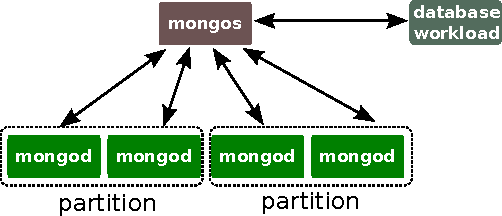
\includegraphics[width=.6\textwidth]{inputs/img/mongo_cluster}
  \caption{MongoDB cluster with five nodes, one query router (mongos) and four node replicas in two partitions (mongod).}
  \label{fig:mongo_cluster}
\end{figure}

The main packages and configuration files of MongoDB cluster are described in Table~\ref{tab:common_install_conf_mm}.

			\begin{table*}[htdp]
				\begin{center}
\caption{Required packages and configuration file adjustments for a MongoDB cluster.}
  \label{tab:common_install_conf_mm}
					\begin{tabular}{R{2.5cm} || L{4.5cm} L{6cm} }
						{\bf Requirement}&{\bf Template/packages}&{\bf Description} \\  
						\hline
						\hline
						{\bf mongos}&\verb|/contrib/debian/mongodb/| \verb|install.sh|, \verb|/contrib/debian/mongodb/| \verb|etc/configdb/mongod.conf|, \verb|/contrib/debian/mongodb/| \verb|etc/qrouter/mongos.conf| & The mongos installation includes a script \verb|install.sh| and two configuration files. While the installation script install the main packages to run both the query router itself and the surrogate configuration daemon, the configuration files are specific to each one of them  and should be adjusted accordingly. \\
						\hline
						{\bf mongod}&\verb|/contrib/debian/mongodb/| \verb|install.sh|, \verb|/contrib/debian/mongodb/| \verb|etc/configdb/mongod.conf| & mongod installation and configuration are straightforward. Basically, the installation requires running the same script for mongos installation and the configuration requires he modification of the DBPATH configuration file variable.\\
					\end{tabular}
				\end{center}
			\end{table*}

Once mongos and mongod are installed and configured properly, the latest step is to add mongod instances to the mongos with the following commands:

\begin{lstlisting}
#once connected to the node running the mongos
sh.addShard( "rs0/primary-mongod-server-partition-0:27017, \
    rs1/primary-mongod-server-partition-1:27017" ) \
sh.shardCollection( "collection.name", 'key': { "_id": "hashed" } ) 
\end{lstlisting}

The first command adds the two primary copies to the query router (mongos) and the second creates a collection of documents whose storage are spread across the nodes according to the hash value of the document keys. After setting-up and configuring the MongoDB cluster, we should load it with data. This step can be performed from the workload by running the following command:

\begin{lstlisting}
sh contrib/debian/mongodb/load.sh
\end{lstlisting}

This script loads a large number of documents into the database cluster. It uses the parameters of \verb|/contrib/debian/mongodb/ycsb-0.1.4/workloads/load|, which can be tuned for particular purposes. Finally, Tejo provides two scripts to run and stop the workload, namely \verb|/tejo/common/experiments_scripts/ycsb/run.sh| and \verb|/tejo/common/experiments_scripts/| \verb|ycsb/stop.sh|.


\subsubsection{VoltDB}

The set-up of a VoltDB cluster differs in two main points from that of MongoDB. First, there is no query router, the workload sends requests directly to nodes that maintain data. Second, its architecture is easier since there is no primary/secondary replica roles, resulting in a simpler deployment. Figure~\ref{fig:voltdb_cluster} depicts a simple VoltDB cluster with four replicas grouped in two partitions.

\begin{figure}[!h]
  \centering
     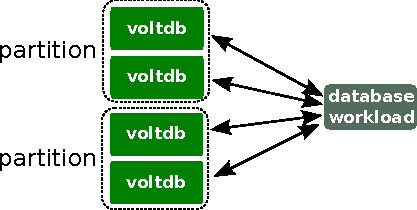
\includegraphics[width=.6\textwidth]{inputs/img/voltdb_cluster}
  \caption{VoltDB cluster with four nodes, four node replicas in two partitions.}
  \label{fig:voltdb_cluster}
\end{figure}

To install VoltDB, one might either clone VoltDB Community Edition from the public repository~\footnote{https://github.com/VoltDB/voltdb/} or download the Enterprise edition for trial~\footnote{http://learn.voltdb.com/DLSoftwareDownload.html}. We recommend the installation of the latter because it includes key features such as high availability that are not currently available in the community edition.

Once the VoltDB is installed in the cluster nodes, the database can be run from the Workload node using the following Tejo's scripts: \verb|/tejo/common/experiments_scripts/tpcc/run.sh| and \verb|/tejo/common/experiments_scripts/tpcc/stop.sh| to use a TPC-C workload~\footnote{http://www.tpc.org/tpcc/detail.asp}, and \verb|/tejo/| \verb|common/experiments_scripts/| \verb|voter-selfcheck/run.sh| and \verb|/tejo/| \verb|common/experiments_scripts/| \verb|voter-selfcheck/stop.sh| for another workload customized for VoltDB clusters.

\subsection{How to configure and use Tejo}
\label{subsec:conftejo}

The configuration and use of Tejo include the following steps: environment set-up, configuration file customization, running the workload and fault injection campaigns, and finally set-up learning/anomaly detection prediction. To illustrate the configuration and use of Tejo, this subsection is based on the deployment example depicted in Figure~\ref{fig:tejo_cluster}, which can be easily extended to larger deployments. As shown in this figure, we assume in this subsection the set-up of a MongoDB cluster with a query router and four data storage nodes as described in \ref{subsub:mongo}.

\begin{figure}[!h]
  \centering
     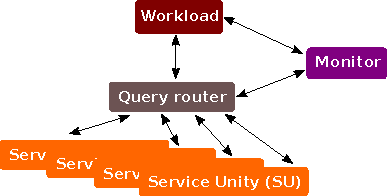
\includegraphics[width=.6\textwidth]{inputs/img/tejo_cluster}
  \caption{Tejo deployment.}
  \label{fig:tejo_cluster}
\end{figure}

\subsubsection{Environment set-up}

The Service Unity (SU) requires the following packages to be installed on your local machine before configuration.

\begin{itemize}
	\item JDK/JRE +1.7~\footnote{http://www.ubuntuupdates.org/openjdk-7-jdk};
	\item Python +2.7~\footnote{http://www.ubuntuupdates.org/python};
	\item gcc/g++ +4.3~\footnote{http://www.ubuntuupdates.org/gcc};
	\item Ant +1.7~\footnote{http://www.ubuntuupdates.org/ant}.
\end{itemize}

In Debian systems, these packages can be installed by running the following packages:

\begin{lstlisting}
sudo apt-get -q -y update 
sudo apt-get -q -y  install git gcc g++ openjdk-7-jdk ant
\end{lstlisting}

In addition to these required packages, nodes in Tejo should be able to communicate directly through OpenSSH without password. First, you should install and set-up a public-private dsa key pair in the Monitoring node as follows:

\begin{lstlisting}
sudo apt-get -q -y install openssh-server
ssh-keygen -t dsa # Please do not enter in a password
cat ~/.ssh/id_dsa.pub >> ~/.ssh/authorized_keys
\end{lstlisting}

Then, the following steps should be performed in the remaining nodes, including SUs and Workload nodes.

\begin{lstlisting}
sudo apt-get -q -y install openssh-server
cat ~/.ssh/id_dsa.pub >> ~/.ssh/authorized_keys
\end{lstlisting}
where \verb|~/.ssh/id_dsa.pub| is the same file initially generated in the Monitor node.
 
\subsubsection{Configuration file}

The file \verb|/etc/tejo.conf| is the main configuration file of Tejo and it should be installed and tuned on each node properly. By cloning the sources from the public repository (described in \ref{subsubsec:gitclone}), you will download a template file whose some key parameters (see Table~\ref{tab:common_install_conf_kp}) should be changed accordingly.

To install the template, run:
\begin{lstlisting}
cp tejo/contrib/tejo/tejo.conf.sample /etc/tejo.conf
\end{lstlisting}

The key parameters to be tuned are:

			\begin{table*}[htdp]
				\begin{center}
\caption{Key parameters of /etc/tejo.conf.}
  \label{tab:common_install_conf_kp}
					\begin{tabular}{R{4cm} || L{6cm} L{3cm} }
						{\bf Parameter}&{\bf Description}&{\bf Examples} \\  
						\hline
						\hline
						{\bf node\_type}&It specifies the role of the node. The possible strings are vm (for SU), monitor, and workload & node\_type=monitor. \\
						\hline
						{\bf location}&This is a parameter that allows Tejo to identify the geographical location of a node. One might set ant string to this parameter. & location=eu, for nodes deployed on European datacenters. \\
						\hline
						{\bf rrd\_path\_vms\_prefix} and {\bf rrd\_path\_workload \_hosts\_prefix}&These are paths to rrd files and should be set only for nodes playing a Monitor role. This path is specific to the operating system. & /var/lib/ganglia/rrds/workload. \\
						\hline
						{\bf guest\_vm\_sys\_user} &Local system user who will deploy and run Tejo.&guest\_vm\_sys\_user= guest\\
						\hline
						{\bf root\_dir} &Path towards which Tejo will be cloned. It is usually the home directory of a system user.&root\_dir= /home/guest\\
						\hline
						{\bf home\_dir} &Destination path of local Tejo repository cloned copy. It is usually inside the home directory of a system user.&home\_dir= /home/guest/tejo\\
						\hline
						{\bf mongo\_query\_ router\_host} &Hostname of the query router.&mongo\_query\_ router\_host= FQDN.of.qrouter\\
						\hline
						{\bf system\_id} &This parameter is specific to the Workload node and describes which kind of systems it is querying.&system\_id= 0, for MongoDB read-only workload, 1 for VoltDB TPC-C, 2 for MongoDB reads and updated, and 3 for VoltDB voter workload.\\
					\end{tabular}
				\end{center}
			\end{table*}

\subsubsection{Workload and fault injection campaigns}

Once the nodes are set-up and configured properly, Tejo provides scripts to run workloads and fault injection campaigns that are easy to perform.

To run a workload, one should run the following script from the Workload node.

\begin{lstlisting}
sh tejo/tejo/common/experiments_scripts/quick_launch/run.sh
\end{lstlisting}

\noindent
this launches requests to SUs. Then, you can launch a fault campaign from the Monitor node as follows.

\begin{lstlisting}
sh tejo/tejo/common/experiments_scripts/quick_launch/inject.sh
\end{lstlisting}

\noindent
this scripts remotely injects faults in SUs by instrumenting \verb|stress-ng| and \verb|dummynet|. Finally, to stop the launched workload, run the following script from the Workload node:

\begin{lstlisting}
sh tejo/tejo/common/experiments_scripts/quick_launch/stop.sh
\end{lstlisting}

Further details about hos to set-up fault injection campaigns are available in our previous work~\cite{silvestre2014anomaly}.

\subsubsection{Set-up learning and anomaly prediction}

The set-up of Tejo for learning and anomaly prediction has two major steps: periodic collection of measurements and data analysis.

The collection of measurements can be performed periodically using the \verb|crontab| of the Monitor node as follows:
\begin{lstlisting}
crontab  -r #to erase the previous jobs
crontab  tejo/data_handler/cron.job
\end{lstlisting}

\noindent
these commands allow us to read rrd files and store them into the PostgreSQL database periodically.

For data analysis, data should be carefully selected from the database, preprocessed and finally put into the learning scripts for selecting raw data, one should get data from two main tables of the PostgreSQL database, namely vm and slo. The following example shows a query template for doing that:

\begin{lstlisting}
select $list_of_columns from vm inner join slo \
           on slo.ts=vm.ts where $filters \
           order by vm.ts;
\end{lstlisting}

This query template defines an aggregated list of comma-separated columns ,\$list\_of\_columns (about 200 columns, including SU/vm resources consumption, SLO performance from the workload, and fault injection activity), selected from a join sql command over the two main tables, vm and slo. \$filters defines the restrictions of our query, mainly concerning the time-stamp column and and fault injection activity.

Once the raw data is collected and stored to a file (either binary-like pickle python or cvs-based text file), you can start preprocessing this data. Preprocessing the raw selected data is very simple and essentially consists in attributing labels to selected lines. Labels definition depends on the learning/prediction tasks. For example, if the goal is to distinguish faulty from fault-free nodes, just two labels are required, e.g. -1 for faulty SU nodes and 1 otherwise.

The latest step of the learning/prediction step is to feed the preprocessed data to the learning script. To this aim, Tejo provides a straightforward, easy-to-customize python script, which contains the definition of a supervised-learning classifier. This file is available on the following Tejo repository path:

\begin{lstlisting}
tejo/learning_model/anomaly_detection.py
\end{lstlisting}

\noindent
this script defines a anomaly detection classifier whose python class is called \verb|OneClassSVMClassifier|. This class is based on Scikit Learning~\footnote{http://scikit-learn.org/}~\cite{scikitlearn11}, an open-source machine learning library, and implements two methods for anomaly detection: the instantiation and the predict method. The former allows us to read the preprocessed file (the training dataset), interpret the attributed labels, and learning anomalous behaviour of faulty nodes. This initial learning phase is run in batch mode. The second, the predict method, can be run on real deployments to predict anomalous SUs. 
\section{Experimental set-up}
\label{sec:experiment}



\subsection{Private cloud set-up}

We performed our experiments on a private cloud consisting of two Dell PowerEdge R620 hosts. Each host has two-core Xeon E5-2660 at 2.2 GHz, 64 GB of memory, and two 130 GB SATA disks. Hosts are connected by Gigabit Ethernet. We chose VMware as the virtualization technology and ESXi 5.1.0 as hypervisor. Figure~\ref{fig:experimental_scenario_extended} depicts our private cloud, highlighting the consolidation of VMs. Each VM of the NewSQL database cluster has 4 GB of memory, 4 CPU cores, a disk of 16 GB, and is connected to a 100Mbps virtual network.

\begin{figure}[!h]
  \centering
     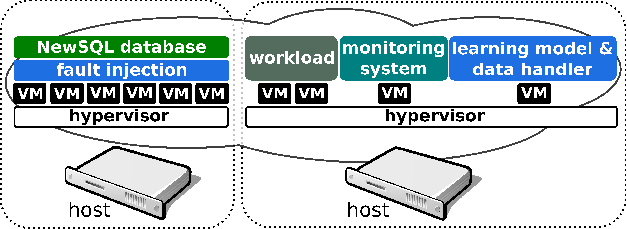
\includegraphics[width=1\textwidth]{inputs/img/experimental_scenario_extended_2}
  \caption{Experimental setup.}
  \label{fig:experimental_scenario_extended}
\end{figure}

\subsubsection{Components of Tejo and monitoring system.} As fault injection tools, we chose Dummynet (v3.0)~\cite{carbone2010dummynet} for network faults and \verb|stress-ng| (v0.01.30)~\footnote{stress-ng. \url{http://kernel.ubuntu.com/~cking/stress-ng/}} for disk, memory, and CPU faults. These tools provide a flexible, easy-to-reproduce way to inject arbitrary fault intensities. Table~\ref{tab:fault_campaign} lists the parameters of our fault injection campaign. The data handler component was implemented as a collection of python/shell scripts along with PostgreSQL database for datasets. We implemented our learning model using the Scikit-learn library~\cite{scikitlearn11}, from which we evaluated three learning algorithms: random forests~\cite{breiman2001random}, gradient boosting~\cite{friedman2006recent}, and SVM~\cite{svm_1995}. We used Ganglia as monitoring system. Our setup required additional Ganglia plug-ins for collecting performance counters of the workload and VoltDB. Every 15 seconds, we collected 147 performance metrics of each VM, and the average throughput and the 99$^{th}$ percentile latency from the served workload. 

			\begin{table*}[htdp]
				\begin{center}
\caption{The key parameters of Tejo for our fault injection campaign.}
  \label{tab:fault_campaign}
					\begin{tabular}{l c || r c c c }
						\multicolumn{2}{ l ||}{\bf Fault}&\multicolumn{3}{ c }{\bf Intensity ranges}&{\bf Unit} \\  
						&&Light&Medium&Heavy& \\  
						\hline
						\hline
						\multirow{3}{*}{\bf Network}&Pkt loss&1.6-3.2&4-5.6&6.4-8&\% \\
						&Latency&8-20&26-38&44-56&ms. \\
						&Limping&85-65&56-38&29-11&Mbps \\
						\hline
						\multicolumn{2}{ l ||}{\bf Memory}&73-79&82-88&91-97&\% \\
						\hline
						\multicolumn{2}{ l ||}{\bf Disk}&10-20&25-35&40-50&writers \\
						\hline
						\multicolumn{2}{ l ||}{\bf CPU}&19-39&49-69&79-99& \% \\
					\end{tabular}
				\end{center}
			\end{table*}



\subsubsection{NewSQL database and workloads.} We evaluated VoltDB (v4.x) as NewSQL database. We set the number of partitions VoltDB to 18 across a cluster of six VMs with failover mechanisms enabled. We varied the replication degree k from two to zero (i.e., replication disabled).  We evaluated VoltDB with two workloads, the popular TPC-C benchmark for OLTP~\footnote{TPC-C benchmark (v5.10). \url{http://www.tpc.org/tpcc/}},  and Voter~\footnote{Voter. \url{https://github.com/VoltDB/voltdb/tree/master/examples/voter.}}, a workload derived from leaderboard maintenance application for Japanese version of the ``American Idol''. We run Tejo for predicting anomalies in MongoDB cluster in our previous work~\cite{silvestre2014anomaly}.


\section{Results}
\label{sec:evaluation}


We evaluate VoltDB, a NewSQL database, with Tejo. First, we describe our experimental setup. Second, we measure the impact of performance anomalies in a VoltDB cluster. Finally, we report on the predictive efficiency of these anomalies.


\subsection{Evaluating performance anomalies in VoltDB}
\label{subsec:performance}

We run Tejo in learning mode(Subsection~\ref{subsec:tejo_phases}) to evaluate the impact of faults in VoltDB. We selected a dataset containing 200,000 samples, including performance counters of VMs and the workload. Data was evenly collected across the two evaluated workloads. Figure~\ref{fig:performance_overview} shows the impact of faults on the performance of VoltDB with a replication degree k=2. For each workload, they show the resulting performance anomalies on the average throughput and 99$^{th}$ percentile latency, including mean values without faults, the expected SLO metrics, and 95\% confidence interval for performance metrics under fault injection. 

Overall, the impact of increasing levels of faults was higher on the 99$^{th}$ percentile latency than the average throughput. For instance, Figure~\ref{fig:fault_impact_this_latency_99th_voltdb_voter} shows that the 99$^{th}$ percentile latency of VoltDB serving Voter workload soars under faults, especially for network and memory faults. Although the mean of the 99$^{th}$ percentile latency without fault was 25 milliseconds, it reaches 945 milliseconds under memory faults. Similar results were found as VoltDB served TPC-C workload. However, we noticed that TPC-C has a greater performance degradation under memory faults (Figure~\ref{fig:fault_impact_this_latency_99th_voltdb_tpcc}). The reason for that is the main memory usage of each workload. While Voter uses 25\% of main memory from each VM, TPC-C utilises almost 50\%. Consequently, TPC-C is more sensitive to memory faults than Voter. Disk faults had a limited impact of the performance of VoltDB, slightly higher on TPC-C than Voter due to a greater need to synchronize data from the main memory to disk (Figure~\ref{fig:fault_impact_this_latency_99th_voltdb_tpcc}). Surprisingly, CPU faults had no impact on the performance of both workloads, even under heavy fault intensity (i.e., 99\% of CPU usage). 

To shed some light on the capacity of data replication to mitigate the impact of performance anomalies, we varied the replication degree k of VoltDB from two to zero (i.e., replication disabled). Figure~\ref{fig:replication_degree_resiliency} shows a summary of the results of the impact of faults with medium intensity on VoltDB. In general, our results suggest that higher the replication degree the worse is the performance. The reason is that NewSQL databases as VoltDB strive to provide ACID properties both for concurrent transactions and for replicas. The impact of a fault on a single node spreads across the replicas on the cluster more easily, worsening its performance.

\begin{figure*}
        \centering
        \begin{subfigure}[b]{0.48\textwidth}
               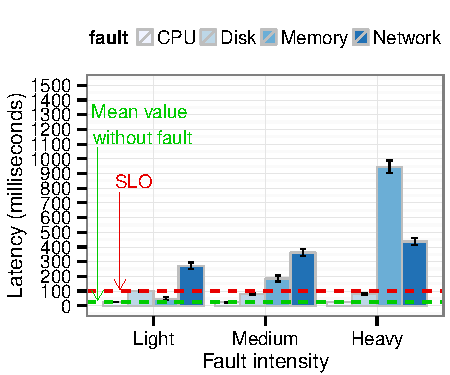
\includegraphics[width=1\textwidth]{inputs/img/fault_impact_this_latency_99th_voltdb_voter}
                \caption{99$^{th}$ percentile latency w/ Voter.}
                \label{fig:fault_impact_this_latency_99th_voltdb_voter}
        \end{subfigure}
        ~ %add desired spacing between images, e. g. ~, \quad, \qquad etc.
        \begin{subfigure}[b]{0.48\textwidth}
                  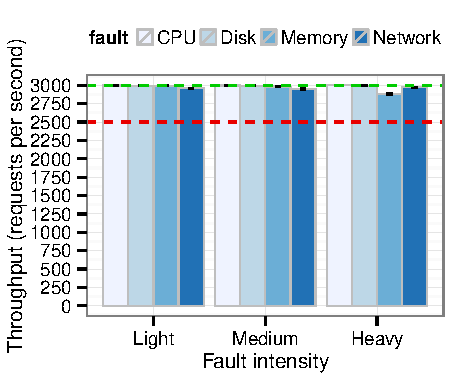
\includegraphics[width=1\textwidth]{inputs/img/fault_impact_this_throughput_voltdb_voter}
                \caption{Average throughput w/ Voter.}
                \label{fig:tejo_overview_detecting}
        \end{subfigure}

        \begin{subfigure}[b]{0.48\textwidth}
                  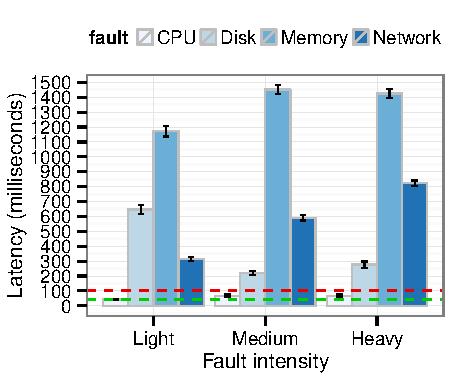
\includegraphics[width=1\textwidth]{inputs/img/fault_impact_this_latency_99th_voltdb_tpcc}
                \caption{99$^{th}$ percentile latency w/ TPC-C.}
                \label{fig:fault_impact_this_latency_99th_voltdb_tpcc}
        \end{subfigure}
	  ~
        \begin{subfigure}[b]{0.48\textwidth}
                  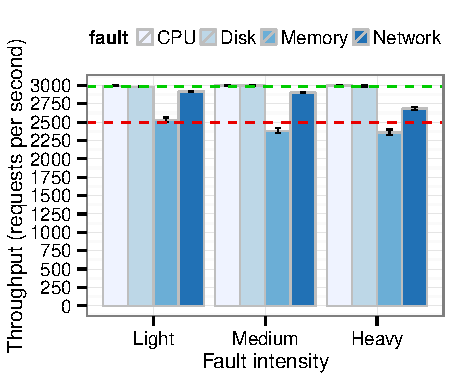
\includegraphics[width=1\textwidth]{inputs/img/fault_impact_this_throughput_voltdb_tpcc}
                \caption{Average throughput w/ TPC-C.}
                \label{fig:fault_impact_this_throughput_voltdb_tpcc}
        \end{subfigure}
        \caption{Performance anomalies in VoltDB as serving Voter and TPC-C, with a replication degree k=2.}
                \label{fig:performance_overview}


\end{figure*}


\begin{figure*}
        \centering
        \begin{subfigure}[b]{0.48\textwidth}
               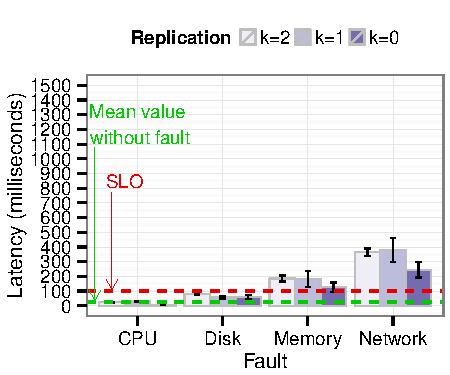
\includegraphics[width=1\textwidth]{inputs/img/k_factor_latency_99th_voltdb_k_analysis_voter}
                \caption{Voter workload.}
                \label{fig:k_factor_latency_99th_voltdb_k_analysis_voter}
        \end{subfigure}
        ~ %add desired spacing between images, e. g. ~, \quad, \qquad etc.
        \begin{subfigure}[b]{0.48\textwidth}
                  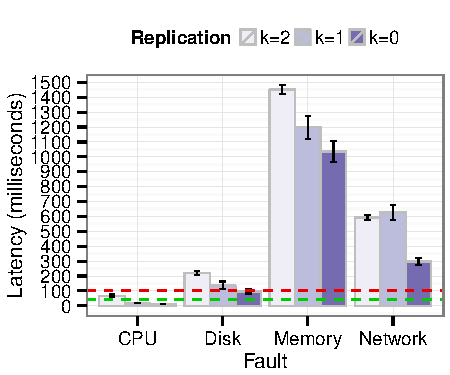
\includegraphics[width=1\textwidth]{inputs/img/k_factor_latency_99th_voltdb_k_analysis_tpcc}
                \caption{TPC-C workload.}
                \label{fig:k_factor_latency_99th_voltdb_k_analysis_tpcc}
        \end{subfigure}
        \caption{Medium fault impact on VoltDB with different k values.}
         \label{fig:replication_degree_resiliency}

\end{figure*}

\subsection{Predictive efficiency analysis}

We evaluated the predictive efficiency of learning model of Tejo with three learning algorithms, random forests, gradient boosting, and SVM. To this end, we used data derived from the dataset of Subsection~\ref{subsec:performance}. The derived data was computed by the Tejo's data handler, as described in Subsection~\ref{subsec:tejo_phases}. Each new sample had 147 features ($d=147$, as discussed in Subsection~\ref{subsec:anomaly}) and a label corresponding to a class of Tejo's learning model (see Subsection~\ref{subsec:tejo_components}). Recall that anomaly-related labels are only assigned to samples that violated the SLO. The resulting dataset contained 10,000 samples for each evaluated workload, including 5,000 of samples representing anomalous events in VMs. To validate the learning model properly, this dataset was split in two uneven parts: three-fifths of data for training the model and two-fifths for testing its predictive efficiency. We used two well-known measures to evaluate the learning model efficiency, precision and F1-score. We also computed the overhead of predictions with each learning algorithm.

Table~\ref{tab:predictive_efficiency} summarizes our results. Regardless the learning algorithm, the learning model of Tejo was able to detect 96\% of anomalies properly. It performed better with random forests algorithm, whose overall score was 0.99 (up to 1) for both precision and F1-score measures. Random forests also provided the lowest overhead for anomaly detection, requiring less than 30 microseconds for a prediction. The SVM algorithm had the worst predictive performance, particularly to detect memory-related anomalies. SVM also incurred the highest overhead for anomaly detection with our model, performing two orders of magnitude slower. According to Friedman~\cite{friedman2006recent}, this happens because SVM shares the disadvantages of ordinary kernel methods, such as poor computational scalability and inability to deal with irrelevant features. In contrast, boosting methods, like random forests and gradient boosting, overcome these issues by using a linear combination of (many) trees.

			\begin{table*}[htdp]
				\begin{center}
\caption{Anomaly detection performance with different learning algorithms.}
  \label{tab:predictive_efficiency}
					\begin{tabular}{r||c | c  c  c  | c  c  c   }
						\multirow{3}{*}{\bf Algorithm}&\multirow{3}{*}{\bf Class}& \multicolumn{6}{ c }{\bf workload} \\ \cline{3-8}
						&&\multicolumn{3}{ c | }{\bf voter}&\multicolumn{3}{ c }{\bf TPC-C} \\ \cline{3-8}
						&&precision&F1-score&overhead&precision&F1-score&overhead \\ 
						\hline
						\hline
						\multirow{3}{*}{\makecell{Random \\  Forests}}&Normal&0.99&0.99&\multirow{3}{*}{23$\mu$s}&0.98&0.99&\multirow{3}{*}{26$\mu$s} \\
						&Network&0.98&0.98&&0.99&0.98& \\
						&Memory&0.99&0.98&&0.98&0.99& \\
						&Disk&0.99&0.98&&1.00&1.00& \\
						\hline
						\multirow{3}{*}{\makecell{Gradient \\ Boosting}}&Normal&0.99&0.99&\multirow{3}{*}{30$\mu$s}&0.96&0.98&\multirow{3}{*}{33$\mu$s} \\
						&Network&0.99&0.99&&0.99&0.96& \\
						&Memory&0.99&0.99&&0.98&0.99& \\
						&Disk&1.00&1.00&&1.00&1.00& \\
						\hline
						\multirow{3}{*}{SVM}&Normal&0.98&0.97&\multirow{3}{*}{4294$\mu$s}&0.98&0.98&\multirow{3}{*}{5441$\mu$s} \\
						&Network&0.97&0.96&&0.99&0.97& \\
						&Memory&0.85&0.91&&0.87&0.93& \\
						&Disk&1.00&0.97&&1.00&1.00& \\
					\end{tabular}
				\end{center}
			\end{table*}

In addition to the predictive efficiency evaluation, Tejo allows us to analyse the importance of features using boosting methods. Figure~\ref{fig:feature_importance_plots} plots the importance of features of the Tejo's learning model, where the sum of all features importances is equal to one.  Figure~\ref{fig:feature_importance} shows the 10 most-important features for anomaly detection in VoltDB serving Voter, seven out of 10 corresponding to performance counters of TCP layer of VMs. This suggests that the peer-to-peer communication pattern among the VoltDB cluster is key for anomaly detection. To provide insights into all 147 features, we organized them into seven distinct categories and measured their grouped importance, as depicted in Figure~\ref{fig:feature_importance_categories}. Indeed, it confirms that features from TCP performance counters form the main category, accounting for more than half the total of importance (0.5345). Surprisingly, the category of VoltDB features had the lowest importance for the anomaly detection task. This suggests that the contribution of database-specific features is negligible, therefore our learning model is likely to have similar predictive performance with different NewSQL databases. Results for TPC-C workload showed a similar trend.

\begin{figure*}
        \centering
        \begin{subfigure}[b]{0.48\textwidth}
               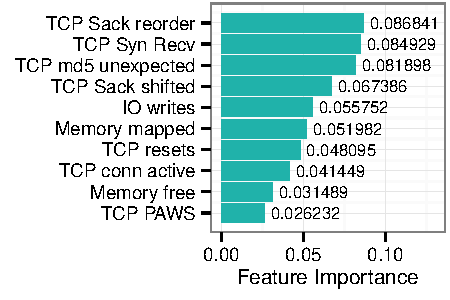
\includegraphics[width=1\textwidth]{inputs/img/feature_importance}
                \caption{The 10 most-important features.}
                \label{fig:feature_importance}
        \end{subfigure}
        ~ %add desired spacing between images, e. g. ~, \quad, \qquad etc.
        \begin{subfigure}[b]{0.48\textwidth}
                  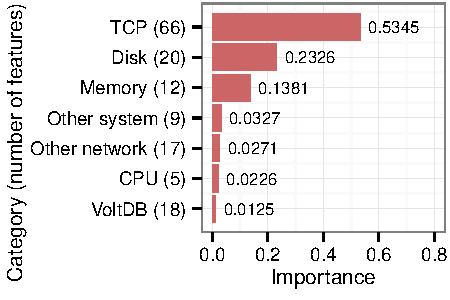
\includegraphics[width=1\textwidth]{inputs/img/feature_importance_categories}
                \caption{Importance of features categories.}
                \label{fig:feature_importance_categories}
        \end{subfigure}
        \caption{Analysis of the importance of features for anomaly detection.}
        \label{fig:feature_importance_plots}
\end{figure*}


\section{Conclusion}
\label{sec:conclusion}

The emerging stream processing platforms rely on NewSQL databases deployed on the cloud to compute big data with high velocity. However, performance anomalies caused by faults on the cloud infrastructure, that are likely to be common, may undermine the capacity of NewSQL databases to handle fast data processing. To analyse these performance anomalies, we proposed Tejo, a supervised anomaly detection scheme for NewSQL databases. This scheme allows us to evaluate the performance of NewSQL database as faults on network, memory, CPU, and disk occur. Experiments with VoltDB, a prominent NewSQL database, showed that the 99$^{th}$ percentile latency soars two orders of magnitude as memory and network faults happen. We showed that Tejo also provides a learning model to detect these performance anomalies. Our findings suggest that learning algorithms based on boosting methods are better to detect anomalies on a VoltDB cluster, and features from the TCP layer of VMs are the best predictors. Results also suggest that the contribution of VoltDB-specific features is negligible, therefore our learning model is likely to have similar efficiency with different NewSQL databases.


%\section{Introduction}

Big data has transformed the way we manage information. As an unprecedented volume of data has become available, there is an increasing demand for stream processing platforms to transform raw data into meaningful knowledge. These velocity-oriented platforms may rely on cloud databases to provide fast data management of continuous and contiguous flows of data with horizontal scalability. Therefore, cloud databases represent an important technology component for a broad range of data-driven domains, including social media, online advertisement, financial trading, security services, and policy-making process.

The architecture of row-store-based relational databases has evolved to meet the requirements of big data on the cloud~\cite{ren2012lightweight}, like elasticity, data partitioning, shared nothing, and especially high performance. The so-called NewSQL databases offer high-speed, scalable data processing in main-memory with consistency guarantees through ACID (atomicity, consistency, isolation, and durability) transactions.

To ensure fast data management, NewSQL databases rely on built-in, fault tolerance mechanisms, like data partitioning, replication, redundant network topologies, load balancing, and failover. Although these mechanisms handle fail-stop failures successfully, many other cloud performance anomalies may remain unnoticed~\cite{server_delays}. For instance, Do \emph{et al.}~\cite{do2013limplock} found that a single limping network interface can cause a three orders of magnitude execution slowdown in cloud databases. Therefore, we believe that the dependability of NewSQL databases might be improved by detecting these anomalies. 

This document proposes Tejo, a supervised anomaly detection scheme for NewSQL databases. We make three specific contributions. First, we introduce a scheme for analysing performance anomalies using fault injection tools and a supervised learning model. Second, we shed some light on the impact of performance anomalies in NewSQL databases. Third, we highlight the importance of selecting the proper features and statistical learning algorithm to enhance the anomaly detection efficiency on these databases.

In the next section, we lay out the recent trends in data stream processing and anomaly detection with statistical learning. Following this, in Section 3 we describe the design of Tejo, in particular its components and its two-phased functioning, namely learning and detection phase. In Section 4 we evaluate VoltDB, a prominent NewSQL database, using Tejo. In our experimental setup, VoltDB served two workloads, whose data was partitioned and replicated across a cluster of virtual machines (VMs). A similar set-up might be done for a MongoDB cluster, as presented in our previous work~\cite{silvestre2014anomaly}. Finally, we discuss the related work in Section 5, and conclude in Section 6.




\addcontentsline{toc}{section}{Bibliography}
\bibliographystyle{plain}
%\begin{thebibliography}{9}
\bibliography{inputs/biblio}
%\end{thebibliography}

\end{document}
